This section describes the research architecture used to answer RQ1--RQ3. The architecture separates data preparation, predictive modeling, evaluation, and explanation analysis while keeping the dataset partitions and experiment configuration consistent across all model families.

\subsection{General Research Pipeline}

The general pipeline consists of the following stages:

\begin{enumerate}
    \item \textbf{Dataset preparation.} The raw healthcare datasets are loaded, normalized, and cleaned. Dataset-specific operations include target cleaning, conversion of invalid zero values to missing values, removal of exact duplicates where appropriate, and identification of numeric and categorical features.
    \item \textbf{Development--test separation.} Each dataset is divided into a stratified 80/20 development--test split using the configured random seed. The test partition is kept untouched until all cross-validation comparisons are complete.
    \item \textbf{Fold construction.} The development partition is divided into five stratified folds. The fold assignment is persisted in \texttt{kfold\_indices.csv} so that AdaBoost, XGBoost, LightGBM, and SHAP analysis use the same validation partitions.
    \item \textbf{Fold-local preprocessing.} For every fold, outlier bounds, imputers, encoders, scalers, and feature selectors are fitted only on the fold-training rows. The fitted transformations are then applied to the corresponding validation rows.
    \item \textbf{Model fitting and prediction.} A fresh model object is created for every dataset, model, and fold. Balanced sample weights are computed from the fold-training labels, and the fitted model produces positive-class probabilities for the validation rows.
    \item \textbf{Predictive evaluation.} ROC-AUC, PR-AUC, Recall, and F1-score are computed for every fold. Mean, standard deviation, minimum, maximum, and range are then aggregated for RQ1 and RQ2.
    \item \textbf{Hold-out evaluation.} After cross-validation, preprocessing is fitted on the complete development partition, each model is refitted, and the final model is evaluated once on the untouched test partition.
    \item \textbf{SHAP analysis.} The same fold assignments are reused for fold-wise SHAP analysis. Feature rankings are compared across folds using Kendall correlation, Spearman correlation, and top-10 Jaccard similarity for RQ3.
\end{enumerate}

The experiment-level settings, including the random seed, split configuration, metrics, model parameters, and SHAP parameters, are stored in \texttt{config.yaml}. The dataset registry in \texttt{src/config.py} stores dataset-specific metadata, while the experiment configuration loader validates the YAML configuration before execution.

\begin{figure}[H]
    \centering
    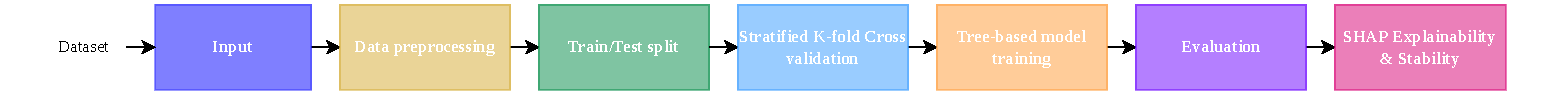
\includegraphics[width=1\linewidth]{pdf/general-pipeline.pdf}\\[10pt]
    \begin{minipage}{0.95\linewidth}
        \begin{figurecaptionmodern}
        \centering
        \capfig{General research pipeline for data preparation, model evaluation, and SHAP-based stability analysis.}
        \label{fig:general-research-pipeline}
        \end{figurecaptionmodern}
    \end{minipage}
\end{figure}

\subsection{Detailed Experimental Pipeline}

The detailed pipeline is implemented through the preprocessing entry point, the model experiment runner, and the SHAP experiment runner. The preprocessing entry point creates reproducible development/test artifacts and the persisted fold assignment. The model runner consumes the raw development rows together with the fold manifest so that every fold can fit its own preprocessing state before training a model. The SHAP runner follows the same fold sequence and explains validation observations using a background derived from the fold-training data.

The detailed implementation pipeline is shown in the following figure.

\begin{figure}[H]
    \centering
    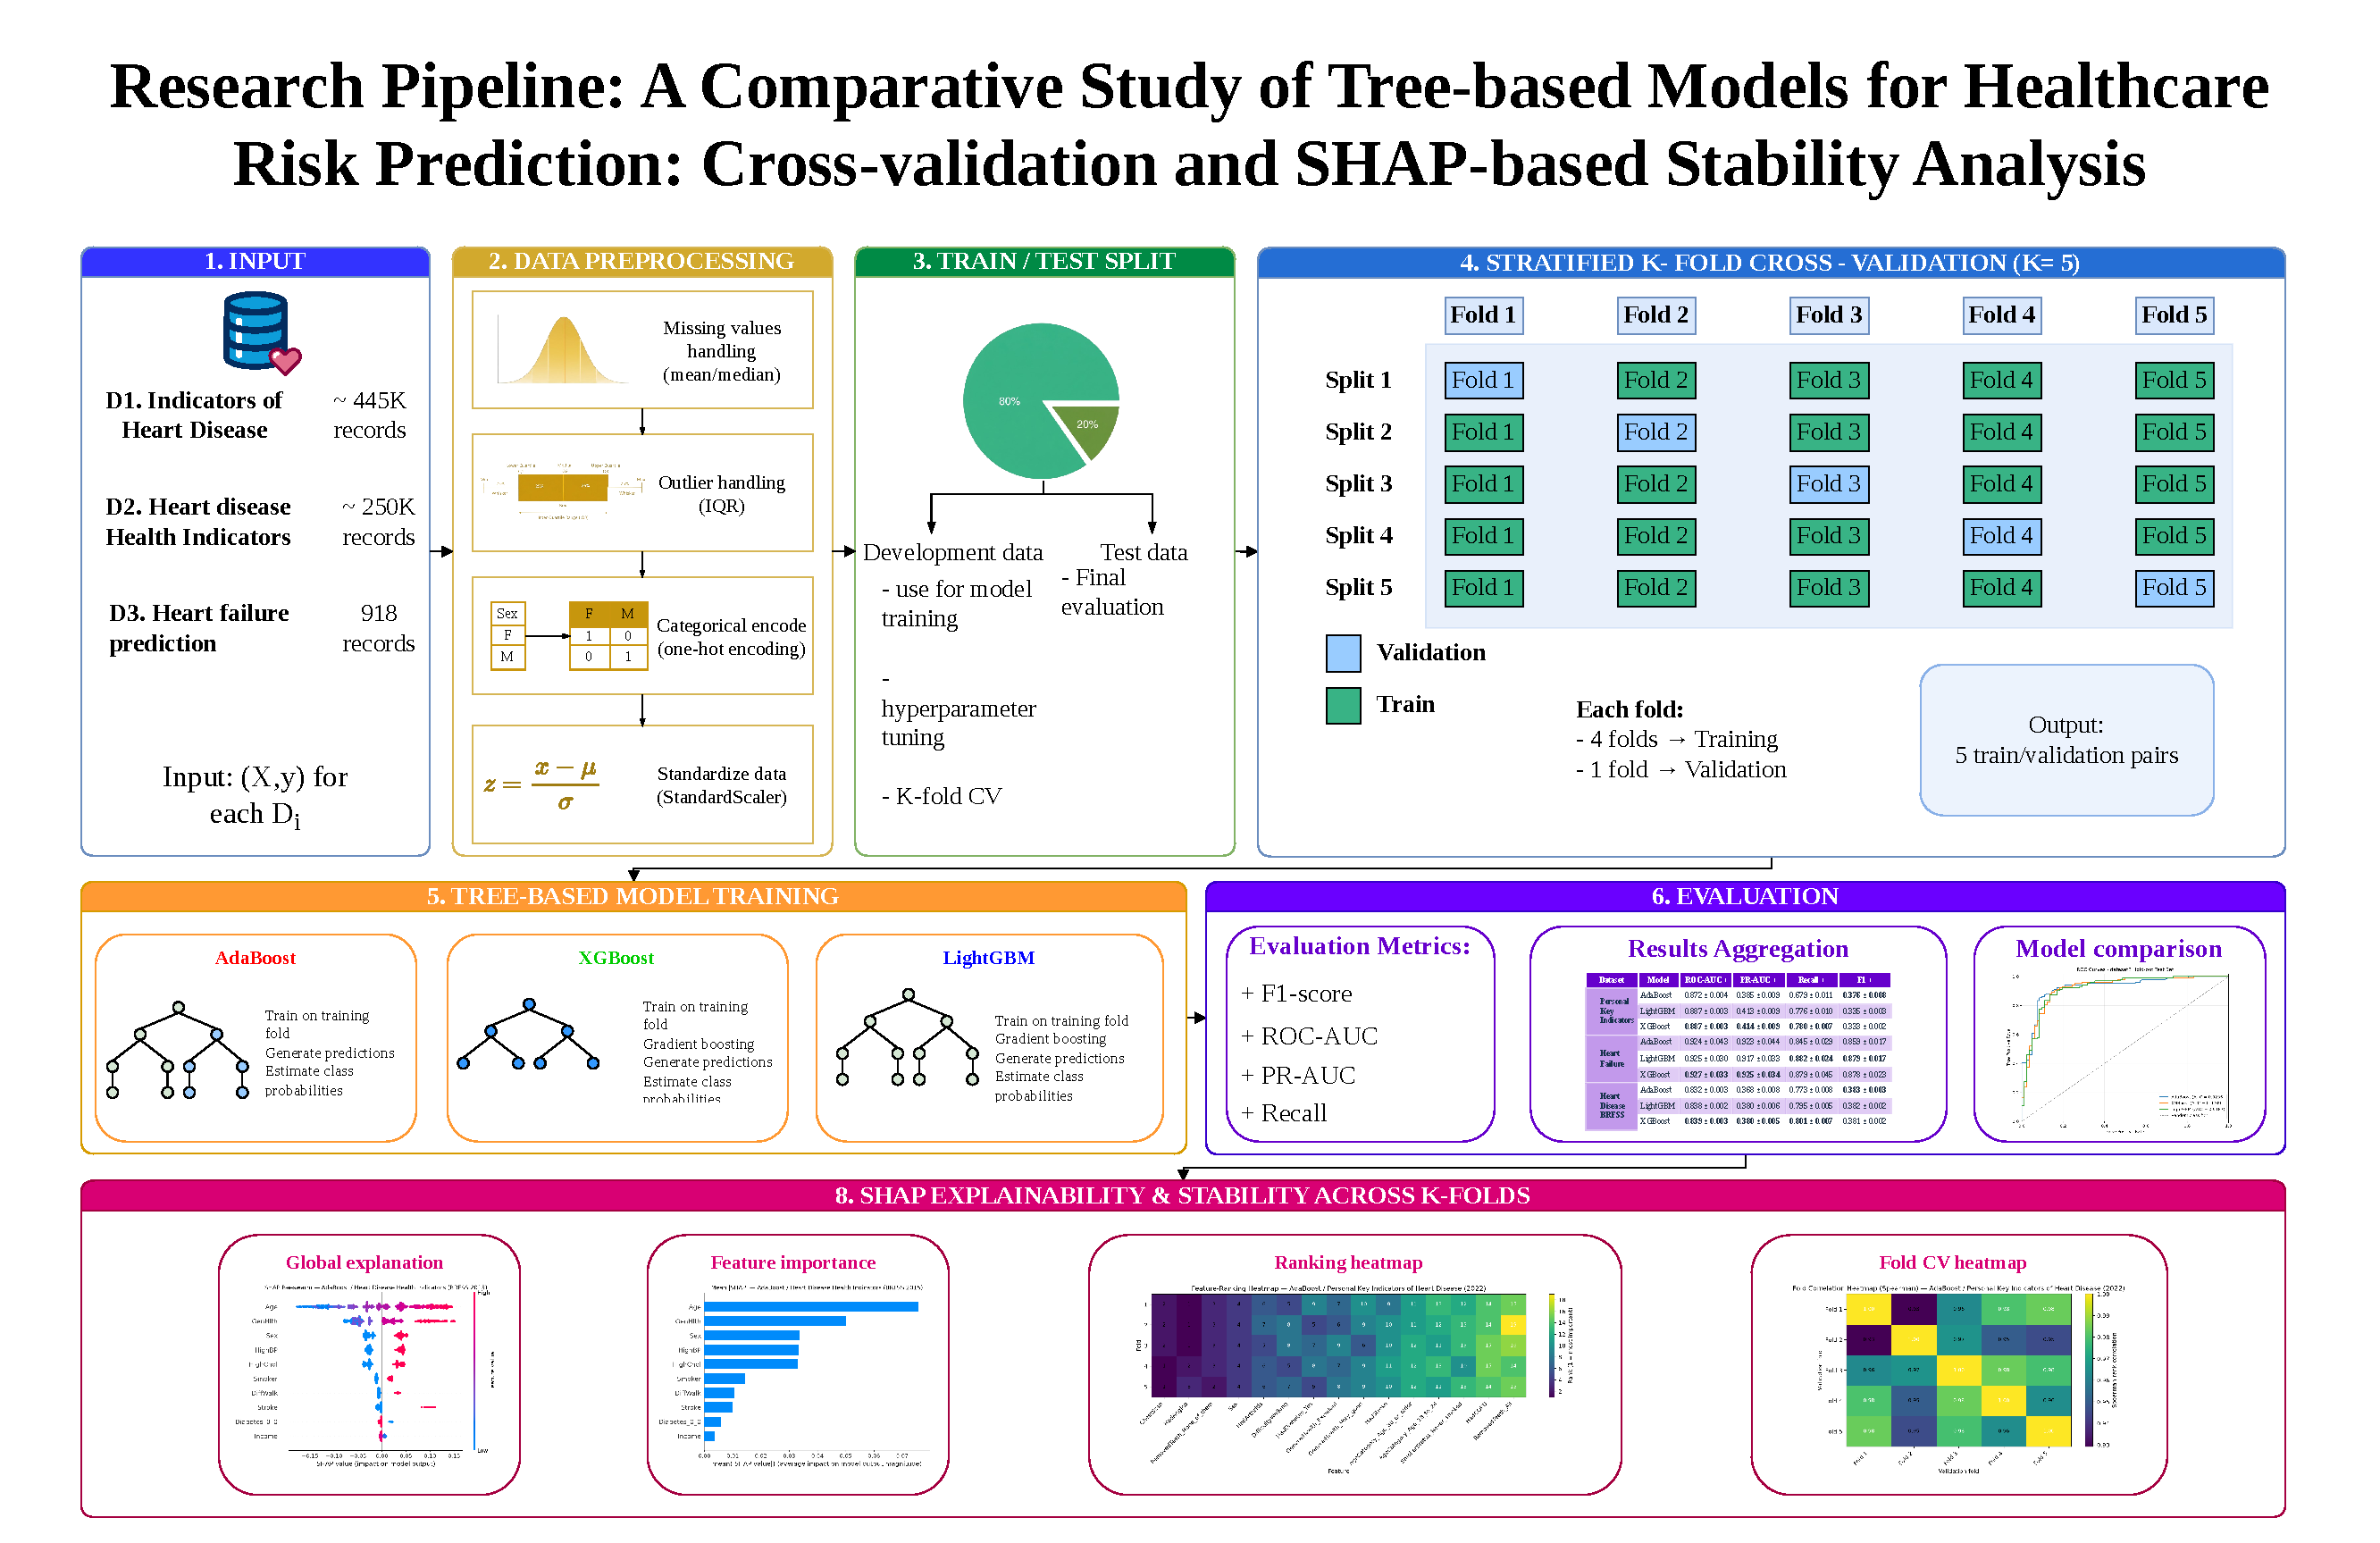
\includegraphics[width=1\linewidth]{pdf/detail-pipeline.pdf}\\[10pt]
    \begin{minipage}{0.95\linewidth}
        \begin{figurecaptionmodern}
        \centering
        \capfig{Detailed implementation pipeline showing fold-local preprocessing, model fitting, hold-out evaluation, and SHAP stability analysis.}
        \label{fig:detailed-research-pipeline}
        \end{figurecaptionmodern}
    \end{minipage}
\end{figure}

\subsection{Research Architecture and Reproducibility}

The architecture deliberately uses fixed model configurations instead of tuning separate configurations for each dataset. This keeps the primary comparison focused on model behavior and fold variability rather than on the variability introduced by repeated hyperparameter searches. It also means that nested cross-validation is not required for the current study design: no model or hyperparameter is selected from the same folds used to report the final stability estimates.

All generated outputs are organized by analysis stage. The model runner writes fold-level metrics, cross-validation summaries, hold-out metrics, rankings, and experiment metadata. The SHAP runner writes fold-level importance values, pairwise stability metrics, consensus rankings, and explainability plots. This separation makes the provenance of each result explicit and allows the report tables and figures to be regenerated from the configured experiment.
